\chapter{Description de la base de données}\label{ch:bd}

La base de données est le cœur du système, c'est elle qui permet la pérennisation des données. L'application mobile peut ensuite exploiter ces données afin de gérer la carte et afficher les diverses informations à l'utilisateur.

Elle est de type PostgreSQL et elle est hébergée directement sur la passerelle.

La base de données permet de stocker les informations suivantes:

\begin{itemize}
\item Information sur les compétiteurs
\item Information sur les compétitions
\item Inscriptions des compétiteurs à des compétitions
\item Enregistrement de chaque paquet de données reçu des capteurs
\end{itemize}

Le diagramme relationnel de la base de données est disponible sur la figure \ref{fig:db_uml}.

\begin{figure}[htb]
\centering 
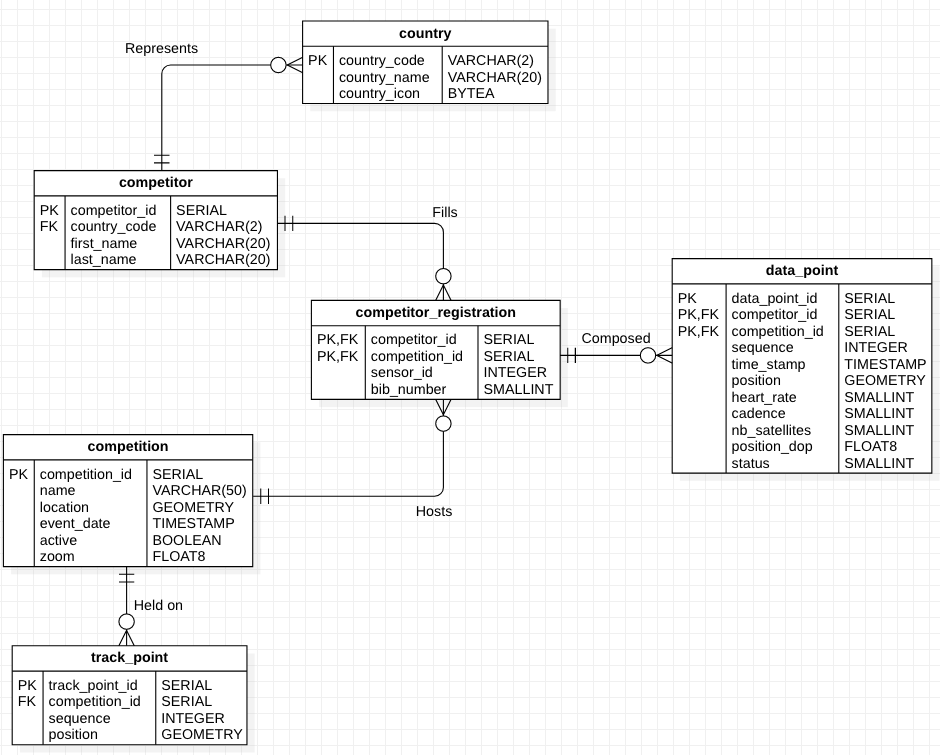
\includegraphics[width=1\columnwidth]{db_uml.png} 
\caption{Diagramme relationnel de la base de données}
\label{fig:db_uml}
 \end{figure}

\section{L'extension PostGIS}

La base de données utilise une extension nommée PostGIS, qui rajoute une série de fonctionnalités qui permettent la gestion d'objet géographique dans la base, ce qui permet de faire des requêtes en utilisant des positions GPS par exemple.

La base de données utilise principalement le type ST\_POINT qui permet de définir des points en spécifiant la latitude et la longitude. Il existe deux types de points différents, geography et geometry. Les points de type geography permettent de prendre en compte la curvature de la planète lors du calcul de distance par exemple. Ce type de point est à préféré lorsque l'application doit faire des opérations entre des points qui sont très éloignés, deux continents différents par exemple. Le type geometry ne prend pas en compte cette information qui complexifie passablement les calculs, mais tire simplement une ligne droite entre les deux points afin de faire le calcul de distance, ce qui convient parfaitement pour des points qui sont faiblement espacés comme c'est le cas pour se travail de Bachelor.

Un exemple de l'utilisation de point est présenté ci-dessous.

\begin{lstlisting}[style=SQLStyle]
INSERT INTO a_table (gps) VALUES (ST_MakePoint(46.9933, 6.91612));

SELECT ST_X(gps) as latitude, ST_Y(gps) as longitude FROM a_table;
\end{lstlisting}

L'extension propose également des fonctions intéressantes comme la possibilité de déterminer la distance entre deux points géographiques.

\begin{lstlisting}[style=SQLStyle]
SELECT ST_Distance(ST_MakePoint(46.9933, 6.91612), ST_MakePoint(46.781036, 6.647138));
\end{lstlisting}

\section{Les tables}

Grâce au modèle relationnel de la base de données ainsi que de l'extension PostGIS, il est ensuite facile d'insérer ou d'extraire des données dans les différentes tables au moyen de requêtes SQL.

Cette section décrit chaque table ainsi que les requêtes SQL qui y sont associées.

\subsection{competition}

Cette table permet de stocker toutes les informations relatives aux compétitions.

\begin{itemize}
\item competition\_id : L'identifiant de la compétition
\item name : Le nom de la course
\item location : L'emplacement de la course. Cette position géographique est utilisée par l'application mobile afin de centrer la vue de la carte correctement
\item event\_date : La date et l'heure du déroulement de la course
\item active : Définit si la course est en direct ou si l'événement est déjà passé
\item zoom : Le zoom que l'application utilise lors du centrage de la vue sur la course
\end{itemize}

La requête SQL suivante définit la façon d'ajouter une nouvelle compétition à la base de données.

\begin{lstlisting}[style=SQLStyle]
INSERT INTO race_tracker.competition (name, location, event_date) VALUES ('Nom de la course', ST_MakePoint(latitude, longitude), '2018-08-01 10:00:00-00');
\end{lstlisting}

Lorsque la passerelle reçoit un paquet de données, elle doit déterminer le competition\_id et le competitor\_id correspondant au coureur qui est défini par le numéro de capteur (sensor\_id). Pour ce faire, la requête suivante est exécutée. Elle permet de trouver le ou les competition\_id du capteur inscrit dans une course qui se déroule actuellement (active = True).

\begin{lstlisting}[style=SQLStyle]
SELECT race_tracker.competitor_registration.competition_id, race_tracker.competitor_registration.competitor_id  FROM race_tracker.competitor_registration INNER JOIN race_tracker.competitor ON (race_tracker.competitor_registration.competitor_id = race_tracker.competitor.competitor_id) INNER JOIN race_tracker.competition ON (race_tracker.competition.competition_id = race_tracker.competitor_registration.competition_id) WHERE race_tracker.competitor_registration.sensor_id = 1234 AND race_tracker.competition.active = True;
\end{lstlisting}

\subsection{competitor}

La table competitor contient tous les sportifs enregistrés dans le système. Une fois enregistrés, ils peuvent participer à des compétitions.

\begin{itemize}
\item competitor\_id : L'identifiant du compétiteur
\item country\_code : Son pays d'origine
\item first\_name : Son prénom
\item last\_name : Son nom de famille
\end{itemize}

Un nouveau compétiteur est rajouté à la base de données en utilisant la requête suivante.

\begin{lstlisting}[style=SQLStyle]
INSERT INTO race_tracker.competitor (first_name, last_name, country_code) VALUES ('Dilyana', 'Petrova', 'BG');
\end{lstlisting}

\subsection{country}

Elle contient tous les pays dont les compétiteur peuvent provenir ainsi que les icônes associés.

\begin{itemize}
\item country\_code : Le code du pays par exemple CH
\item country\_name : Le nom du pays
\item country\_icon :  L'icône représentant le drapeau du pays
\end{itemize}

Un pays est rajouté grâce à la requête suivante.

\begin{lstlisting}[style=SQLStyle]
INSERT INTO race_tracker.country VALUES ('BG', 'Bulgaria', bytea('country/bulgaria.svg'));
\end{lstlisting}

\subsection{competitor\_registration}

La table competitor\_registration permet d'effectuer l'inscription des sportifs à une compétition.

\begin{itemize}
\item competitor\_id : L'identifiant du compétiteur inscrit
\item competition\_id : L'identifiant de la compétition auquel le compétiteur est inscrit
\item sensor\_id : L'identifiant du capteur que le compétiteur porte pendant la course. Cet identifiant est envoyé dans tous les paquets envoyés par le capteur
\item bib\_number : Le numéro de dossard du compétiteur
\end{itemize}

Une inscription s'effectue de la manière suivante.

\begin{lstlisting}[style=SQLStyle]
INSERT INTO race_tracker.competitor_registration (competitor_id, competition_id, sensor_id, bib_number) VALUES (1, 1, 1234, 57);
\end{lstlisting}

L'application mobile a besoin de savoir tous les concurrents qui sont inscrits à une certaine course, la requête suivante permet de récupérer ces informations.

\begin{lstlisting}[style=SQLStyle]
SELECT * FROM race_tracker.competitor_registration INNER JOIN race_tracker.competitor ON (competitor_registration.competitor_id = competitor.competitor_id) WHERE competitor_registration.competition_id = 1;
\end{lstlisting}

\subsection{data\_point}

Chaque data point correspond à un paquet émis par un capteur et contient toutes les informations. L'application mobile exploite les data points afin de pouvoir afficher les informations à l'utilisateur.

\begin{itemize}
\item data\_point\_id : Identifiant du data point
\item competitor\_id : Identifiant du compétiteur dont le data point provient
\item competition\_id : L'identifiant de la compétition à laquelle le data point est rattaché
\item sequence : Un numéro de séquence qui est envoyé dans le paquet. Cette information permet de savoir si des paquets ont été perdus lors de la transmission
\item time\_stamp : Le timestamp envoyé dans le paquet qui correspond au moment de la génération du paquet
\item position : La position GPS du compétiteur
\item heart\_rate : Le rythme cardiaque du compétiteur
\item cadence : La cadence du compétiteur
\item nb\_satellites : Le nombre de satellites en vue au moment de la génération du paquet
\item position\_dop : Dissolution of precision, c'est à dire le degré de certitude de la précision de la position GPS
\item status : L'état du capteur au moment de la génération du paquet
\end{itemize}

La requête suivante permet d'ajouter un nouveau data point dans la base de données. Cette opération est effectuée par la passerelle à chaque fois qu'un nouveau paquet est reçu.

\begin{lstlisting}[style=SQLStyle]
INSERT INTO race_tracker.data_point (competitor_id, competition_id, sequence,position, time_stamp) VALUES (1, 2, 1, ST_MakePoint(46.7856, 6.6424), '2018-10-15 00:00:00');
\end{lstlisting}

Durant son exécution, l'application mobile va exécuter périodiquement une requête, qui permet de connaître le numéro de séquence du dernier data point pour chaque concurrent inscrit à une certaine compétition. La requête suivante permet d'effectuer cette opération. Cette requête est en fait deux requêtes imbriquées, la première permet l'affichage de toutes les informations du data point du point contenant le numéro de séquence le plus élevé pour chaque concurrent (WHERE therank = 1), la deuxième va récupérer tous les data point et les trier par ordre décroissant.

\begin{lstlisting}[style=SQLStyle]
SELECT data_point_id, competitor_id, competition_id, sequence, time_stamp, ST_X(position) as lat, ST_Y(position) as lon, heart_rate, cadence, nb_satellites, position_dop, status FROM (SELECT rank() OVER (PARTITION BY data_point.competitor_id ORDER BY sequence DESC) AS therank, * FROM race_tracker.data_point WHERE data_point.competition_id = 1) t WHERE therank = 1;
\end{lstlisting}

\subsection{track\_point}

Les track point correspondent à chaque point qui constitue le tracé de la course, l'application mobile va connecter chaque point par une ligne ce qui permettra de dessiner le tracé de la course sur la carte.

\begin{itemize}
\item track\_point\_id : Identifiant du track point
\item competition\_id : L'identifiant de la compétition du track point
\item sequence : Le numéro de séquence du track point
\item position : La position géographique du point
\end{itemize}

Un nouveau track point peut être rajouté très simplement grâce à la requête suivante.

\begin{lstlisting}[style=SQLStyle]
INSERT INTO race_tracker.track_point (competition_id, sequence, position) VALUES (3, 1, ST_MakePoint(46.7856, 6.6424));
\end{lstlisting}
